\documentclass[12pt,aspectratio=53,mathserif]{beamer}		
%设置为 Beamer 文档类型,设置字体为 10pt,长宽比为16:9,数学字体为 serif 风格
%%%%%%%%%%%%%%%%%%%%%% 主题 %%%%%%%%%%%%%%%%%%%%%%%%%
\usetheme{Boadilla}
%%%%%%%%%%%%%%%%%%%%%%%%%%%%%%%%%%%%%%%%%%%%%%%%%%%
%%%%-----导入宏包-----%%%%
\usepackage{ctex}%显示中文的包
\usepackage{amsmath,amsfonts,amssymb,bm}   %导入数学公式所需宏包
\usepackage{color}			 %字体颜色支持
\usepackage{graphicx,hyperref,url}	
\usepackage{verbatim}
\usepackage{booktabs}
\usepackage{tikz}
\tikzstyle{arrow}     = [thick,->,>=stealth]
\usepackage{hyperref}
\usepackage{pstricks}
\usepackage{setspace}
\usepackage{pstricks-add}
\tracingmacros=1
%\pdfcompresslevel=0
\hypersetup{
	colorlinks=ture,
	linkcolor=blue,
	filecolor=gray,
	urlcolor=blue,
	citecolor=blue}
%%%%%%%%%%%%%%%%%%
\usepackage[backend=bibtex,sorting=none]{biblatex}
%\addbibresource{bibtex.bib} %BibTeX数据文件及位置
\setbeamerfont{footnote}{size=\scriptsize}
%%%%%%%%%%%%%%%  目录    %%%%%%%%%%%%%%%%%%%%%%%%%%

\AtBeginSection[]
{
  \begin{frame}<beamer>
    \frametitle{\textbf{Outline}}
    \textbf{\tableofcontents[currentsection]}
  \end{frame}
}

%%%%%%%%%%%%%%%%%%%%%%%%%%%%%%%%%%%%%%%%%%%%%%%%%%%%%%

%%%%%%%%%%%%%%%%%%%%%%%%%%%%%%%%%%%%%%%%%%%%%%%%%%%%%%%%

%%%%----首页信息设置----%%%%

\title[Higher Gauge Theory based on Crossed module ]   %底部显示 
       {\textbf{Higher Gauge Theory based on Crossed module} }   %标题
      
%\subtitle{项目名称}


\author[Capital Normal University]    %底部显示
       {Repoter:MengYao Wu
       	\\[3mm]}
   


\date[2023年3月18日]{2023年3月18日}
%%%%----日期信息

\begin{document}

\begin{frame}
\titlepage
\end{frame}				%生成标题页



	
%	\section{Background and Motivation}
%	
%	\begin{frame}
%	\frametitle{Background and Motivation}
%	\begin{itemize}
%		\item Gauge theory
%		\item Higher gauge theory
%		\footnote{ J. C. Baez, J. Huerta, An invitation to higher gauge theory, Gen. Relativ. Gravit. 43 (2010) 2335–2392, \href{arXiv:1003.4485}{arXiv:1003.4485}.}
%	\end{itemize}
%	
%	\end{frame}

	\section{Gauge Theory}
	
        
    
	\begin{frame}{Gauge Theory}
		\begin{itemize}
            \begin{spacing}{2.0}
			\item 
			Category, Lie group.
			
			\ 
			\item 
			 Parallel transport,principal bundle, connections.
		\end{spacing}
    	\end{itemize} 
  	\end{frame}

\begin{frame}{Category}
    	\begin{enumerate} 
        \item Objects
        $$x \bullet$$
        \item Morphisms
        $$\begin{tikzpicture}
            \node[black](a)at(0, 0){$x \bullet$};
            \node[black](b)at(4, 0){$\bullet y $};
            \draw[<-](a)to [bend left=45](b);
            \node[black](c)at(2, 1.2){$f$};
        \end{tikzpicture}$$
        \item Composite morphism
    $$\begin{tikzpicture}
        \node[black](a)at(0, 0){$x \bullet $};
        \node[black](b)at(3, 0){$\bullet y $};
        \node[black](c)at(6, 0){$\bullet z $};
        \draw[<-](a)to [bend left=45](b);
        \draw[<-](b)to [bend left=45](c);
        \node[black](d)at(1.5, 1.2){$f$};
        \node[black](e)at(4.5, 1.2){$g$};
    \end{tikzpicture}$$
 \item Identity morphism $1_x:x\rightarrow x$ 
    \end{enumerate}
  \end{frame}
	
	
\begin{frame}
    {Example}
    \begin{itemize}
        \item Sets is the category whose objects are sets and whose morphisms are functions.
        \item Top is the category of topological spaces and continuous maps.
        \item SmoothMfld is the category of smooth manifolds and smooth maps.
        \item Group
    \end{itemize}
\end{frame}


\begin{frame}
    {Functor between category C and D}
    \begin{enumerate}
        \item \text{$F$ sending objects in C to objects in D,}
        \item \text {$F$ sending morphisms in C to morphisms in D,such that}\\
        given a morphism $f:x \rightarrow y $ in C,we have:$F(f):F(x) \rightarrow  F(y),$
        \item \text{$F$ preserves composition:}
        $F(fg)=F(f)F(g)$ 
        \text{when either side is well-defined,and}
        \item \text{$F$ preserve identityes:}
        $F(1_x)=1_{F(x)}$
        \text{for every object $x$ of C}
    \end{enumerate}
\end{frame}

\begin{frame} 
    {Principle Bundle}
   \begin{enumerate} 
           \item \text {Bundle manifold P,Base manifold M,Structure group G,satisfied}
           \item \text {An free right action $R:P \times G \rightarrow G;$}
           \item \text {An $C^{\infty},onto map:\pi:P \rightarrow M,\pi^{-1}[\pi(p)]={pg,g\in G},\forall p \in P$;}
           \item \text{$\forall x$, there are  open  neighborhoods $U\in M$ and differential isomorphisms,}
           \item \text{$ T_U:\pi^{-1}[U] \rightarrow U \times G\quad T_U(p)=(\pi(p),S_U(p)),$ and}\\
          \text{$S_U(pg)=S_U(p)g,\quad \forall g \in G$}
       \item \text{Trival bundle over M ,$P = M \times G $}
       \end{enumerate}
\end{frame}

\begin{frame}
     {Three equivalent representations of a connection}
     \newtheorem{mythm}{Theorem}
     \begin{mythm}\label{cc}
        For any Lie group G and any smooth manifold M,there is a one to one correspondence between:\\
        1:connections on the trival principle G-bundls over M,\\
        2:$\mathfrak{g}$-valued 1-forms on M,where $\mathfrak{g}$ is the Lie algebra of G,and\\
        3:smooth functors:
    \begin{align*}
    hol :\mathcal{P}_1(M) \rightarrow G
\end{align*}
       where $\mathcal{P}_1(M)$ is the path groupoid of M
     \end{mythm}
\end{frame}

\begin{frame}
    {The construction of $\mathcal{P}_1(M)$ }
    \begin{itemize}
        \item Objects are points of $M$.
        \item Morphisms are thin homotopy classes of lazy paths in $M$.
        \item composotion $[\gamma][\delta]=[\gamma \delta]$.
        \item $\forall x \in M$,the identity $1_x$ is the thin homotopy class of the constant path ay $x$.
         \end{itemize}
     \item \text{A path is lazy if it is smooth and also constant in a neiborhood of t=0 and t=1.}
     \item \text{A hotomopy is thin if it sweeps out a surface that has zero area.}
\end{frame}

\begin{frame}
    {The equivalent between the second and third of Theorem }
    \begin{enumerate}
         \begin{align}
             hol(\gamma)=\mathcal{P}exp(\int_{\gamma} A)
            \end{align}
        \begin{align}
            \gamma:[0,1] \rightarrow M
        \end{align}
             \begin{align}
                \gamma_s:[0,s] \rightarrow M
             \end{align}
             \begin{align}
                 A(v)=\left.\frac{d}{ds}hol(\gamma_s)\right|_{s=0}
             \end{align}
        $v$ is any tangent vector at a point $x \in M,\gamma $ is any smooth path with
        \begin{align}
            \gamma(0)=x,\gamma'(0)=v.
        \end{align}
    \end{enumerate}
        \end{frame}
    
\begin{frame}
    {$T$}
     \end{frame}


\begin{frame}{$U(1)$-Electromagnetism}         
    \begin{enumerate}
        \item Maxwell's Equation 
               $$ \begin{cases}
                    \nabla\cdot\vec{B}=0\\
                    \nabla\times\vec{E}+\frac{\partial\vec{B}}{\partial t}=0\\
                    \nabla\cdot\vec{E}=\rho \\
                    \nabla\times\vec{B}-\frac{\partial\vec{E}}{\partial t}=\vec{j}
                \end{cases}$$\\
                \item Maxwell's Equation in differential form
                $$\begin{cases}
                    dF=0\\
                    *d*F=J
                \end{cases}$$
        \item $F=dA$ $A$ is a $\mathfrak{g}$-valued 1-forms on M.
    \end{enumerate} 
\end{frame}


	\section{2-Gauge Theory}

\begin{frame}{2-Guage Theory}
    \begin{itemize}
        \begin{spacing}{2.0}
          
        \item %范畴,主丛,平行移动,联络,李群
       2-Category, Lie 2-group(crossed module).
        
        \ 
        
        %	\pause
        \item 
        %			\footnote{ J. C. Baez, U. Schreiber, Higher gauge theory, Contemp. Math. 431 (2007) 7–30, \href{arXiv:math/0511710}{arXiv:math/0511710}.}
        %			\footnote{J. C. Baez, U. Schreiber, Higher gauge theory: 2-connections on 2-bundles, \href{	arXiv:hep-th/0412325}{	arXiv:hep-th/0412325}},
        %主2-丛,2-平行移动,2-联络,李2-群
         2-parallel transport, principal 2-bundle, 2-connections.
        %			
        %			\ 
        %			
        %			\pause \item 
        %%			\footnote{W. Wang, On 3-gauge transformations, 3-curvatures, and Gray-categories, J. Math. Phys 55 (2014) 043506, \href{arXiv:1311.3796}{arXiv:1311.3796}}, 
    \end{spacing}
    \end{itemize}
    
\end{frame}
	
   \begin{frame}{\color{blue}2-category}
			\begin{enumerate} 
			\item
		    $$\bullet$$
		    \item
		     $$\begin{tikzpicture}
		    	\node[black](a)at(0, 0){$\bullet $};
		    	\node[black](b)at(4, 0){$\bullet $};
		    	\draw[<-](b)to [bend right=45](a);
		    	\node[black](c)at(2, 1.2){$f$}
		    \end{tikzpicture}$$
	    \item
  $$\begin{tikzpicture}
	\node[black](a)at(0, 0){$\bullet $};
	\node[black](b)at(4, 0){$\bullet $};
		\node[black](c)at(2, 1.2){$f$};
			\node[black](c)at(2, -1.2){$g$};
	\draw[<-](b)to [bend left=45](a);
	\draw[<-](b)to [bend right=45](a);
	\node[black]at(2. 2, 0. 0){$\alpha$}
	\node[black]at(1. 9, 0. 0){$\Downarrow $};
\end{tikzpicture}$$
		
			\end{enumerate} 
			\end{frame}
         
		\begin{frame}
         \item \text {2-morphism can be composed in two distinct ways,vertically }
         \begin{enumerate}
             $$\begin{tikzpicture}
                
                    \node[black](a)at(0, 0){$\bullet $};
                    \node[black](b)at(4, 0){$\bullet $};
                    \node[black](e)at(5, 0){$=$};
                    \node[black](e)at(7, 0){$\bullet $};
                    \node[black](f)at(9, 0){$\bullet $};
                    \node[black](c)at(2, 1.2){$f$};
                    \node[black](c)at(2, -1.2){$f''$};
                    \node[black](c)at(1.5, 0.2){$f'$};
                    \draw[<-](a)to [bend left=45](b);
                    \draw[<-](a)to [bend right=45](b);
                    \draw[<-](a)to [bend right=0](b);
                    \node[black]at(2. 2, 0.5){$h$}
                    \node[black]at(2. 2, -0.5){$h$}
                    \node[black]at(1. 9, -0.5){$\Downarrow $};
                    \node[black]at(1. 9, 0.5){$\Downarrow $};
                    \node[black](c)at(8, 0.8){$f$};
                    \node[black](c)at(8, -0.8){$f''$};
                    \draw[<-](e)to [bend left=45](f);
                    \draw[<-](e)to [bend right=45](f);
                    \node[black]at(8. 3, 0. 0){$h'\cdot h$}
                    \node[black]at(7. 7, 0. 0){$\Downarrow $};
                \end{tikzpicture}$$ 
            
         \end{enumerate}
         
      \end{frame}

\begin{frame}
    \item \text {horizontally }
    \begin{enumerate}
        
        $$\begin{tikzpicture}
            \node[black](a)at(0, 0){$\bullet $};
            \node[black](b)at(2, 0){$\bullet $};
            \node[black](c)at(4, 0){$\bullet $};
            \node[black](d)at(5, 0){$= $};
            \node[black](e)at(6, 0){$\bullet $};
            \node[black](f)at(10, 0){$\bullet $};
            \node[black](g)at(1, 0.8){$f_1$};
            \node[black](h)at(1, -0.8){$f'_1$};
            \node[black](i)at(3, 0.8){$f_2$};
            \node[black](j)at(3, -0.8){$f'_2$};
            \node[black](i)at(8, 1.2){$f_1f_2$};
            \node[black](j)at(8, -1.2){$f'_1f'_2$};
            \draw[<-](a)to [bend left=45](b);
            \draw[<-](a)to [bend right=45](b);
            \draw[<-](b)to [bend left=45](c);
            \draw[<-](b)to [bend right=45](c);
            \draw[<-](e)to [bend left=45](f);
            \draw[<-](e)to [bend right=45](f);
            \node[black]at(1. 2, 0. 0){$h_1$};
            \node[black]at(0. 9, 0. 0){$\Downarrow $};
            \node[black]at(3. 2, 0. 0){$h_2$};
            \node[black]at(2. 9, 0. 0){$\Downarrow $};
             \node[black]at(8. 2, 0. 0){$h_1\circ h_2$};
            \node[black]at(7.5, 0. 0){$\Downarrow $}
          
          
        \end{tikzpicture}$$
        
    \end{enumerate}
    
\end{frame}

 \begin{frame}
    \begin{enumerate}
        \item \text{$\forall f$, An identity for vertical composotion $1_f$ }
        \item \text{An identity for horizontal composotion $1_{1_x}$ }
        \item \text{the interchange law:$(h'_1 \cdot h_1)\circ(h'_2 \cdot h_2)=(h'_1 \circ h'_2) \cdot (h_1 \circ h_2)$ }
    \end{enumerate}  
 \end{frame}

\begin{frame}
    {2-Functor}
    \begin{enumerate}
        \item \text {given a 2-morphism $\alpha:f \rightarrow g $ in C,we have:$F(\alpha):F(f) \rightarrow  F(g),$}
        \item \text{F preserves vertical and horizontal composition for 2-morphisms,}\\
           \text  {and indentity 2-morphisms:}\\
        \begin{align}
          F(\alpha \beta)=F(\alpha)F(\beta)
        \end{align}
    \begin{align}
          F(\alpha \circ \beta)=F(\alpha) \circ F(\beta)
       \end{align} 
   \begin{align}
          F(1_f)=1_{F(f)}
        \end{align}
    \end{enumerate}
\end{frame}
  
  
        \begin{frame}{Crossed module}
            {\color{blue} Lie crossed modules $\longleftrightarrow$ Lie 2-groups}
            %	\pause
            %\begin{definition}
            A crossed module $\left(H,G;\alpha,\vartriangleright \right)$:
            
            \begin{itemize}
                \item  groups: $G$, $H$
                \item a group map $\alpha: H  \longrightarrow G$
                \item a action $\vartriangleright$ of G on H by automorphisms
            \end{itemize}
            such that:
            \begin{equation}
                \alpha \left(g \vartriangleright h\right) = g \alpha \left(h\right) g^{-1}, \ \ \ \ \ \ \ \forall g \in G , h \in H,
            \end{equation}
            \begin{equation}
                \alpha \left(h\right) \vartriangleright h' = h h' h^{-1}, \ \ \ \ \ \ \ \forall h, h' \in H.
            \end{equation}
            
            %	\end{definition}
        %	\pause
        {\color{red} Differential crossed modules $(\mathfrak{h}, \mathfrak{g}; \alpha, \vartriangleright)$ $\longleftrightarrow$ Lie 2-algebras }
    \end{frame}


  \begin{frame}
      {2-group $\mathcal{G} \Longrightarrow $crossed module $\left(H,G;\alpha,\vartriangleright \right)$}
      \begin{enumerate} 
      \item \text{G is the set of morphism in $\mathcal{G}$ with composition as the group operation.}
      \item \text{H is the set of all 2-morphism whose source is identity }\\
      \text{with horizontal composition.}
      \item \text{A group homomorphism $\alpha:H \rightarrow G$ sending each 2-morphism in H to its target:}
       $$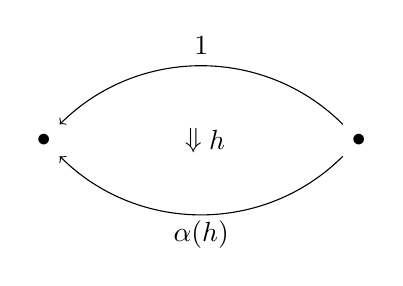
\begin{tikzpicture}
          \node[black](a)at(0, 0){$\bullet $};
          \node[black](b)at(4, 0){$\bullet $};
          \node[black](c)at(2, 1.2){$1$};
          \node[black](c)at(2, -1.2){$\alpha(h)$};
          \draw[<-](a)to [bend left=45](b);
          \draw[<-](a)to [bend right=45](b);
          \node[black]at(2. 2, 0. 0){$h$};
          \node[black]at(1. 9, 0. 0){$\Downarrow $};
      \end{tikzpicture}$$
       \end{enumerate} 
    \end{frame}
      
     
      
       \begin{frame} 
        \item \text{$g \vartriangleright h:$}
        $$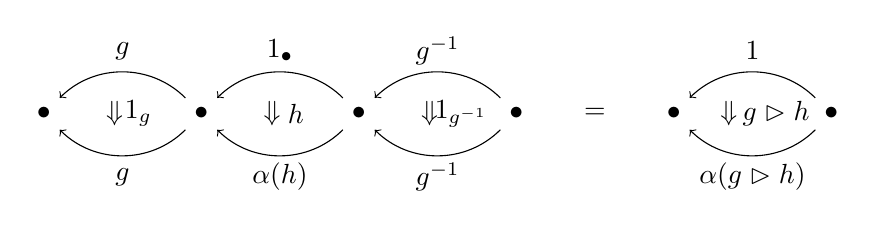
\begin{tikzpicture}
           \node[black](a)at(0, 0){$\bullet $};
           \node[black](b)at(2, 0){$\bullet $};
           \node[black](c)at(4, 0){$\bullet $};
           \node[black](d)at(6, 0){$\bullet $};
           \node[black](e)at(1, 0.8){$g$};
           \node[black](f)at(1, -0.8){$g$};
           \node[black](g)at(3, 0.8){$1_\bullet$};
           \node[black](h)at(3, -0.8){$\alpha(h)$};
           \node[black](i)at(5, 0.8){$g^{-1}$};
           \node[black](j)at(5, -0.8){$g^{-1}$};
           \draw[<-](a)to [bend left=45](b);
           \draw[<-](a)to [bend right=45](b);
           \draw[<-](b)to [bend left=45](c);
           \draw[<-](b)to [bend right=45](c);
           \draw[<-](c)to [bend left=45](d);
           \draw[<-](c)to [bend right=45](d);
           \node[black]at(1. 2, 0. 0){$1_g$};
           \node[black]at(0. 9, 0. 0){$\Downarrow $};
           \node[black]at(3. 2, 0. 0){$h$};
           \node[black]at(2. 9, 0. 0){$\Downarrow $};
           \node[black]at(5. 3, 0. 0){$1_{g^{-1}}$};
           \node[black]at(4. 9, 0. 0){$\Downarrow $};
           \node[black](k)at(7, 0){$=$};
           \node[black](m)at(8, 0){$\bullet $};
           \node[black](n)at(10, 0){$\bullet $};
           \draw[<-](m)to [bend right=45](n);
           \draw[<-](m)to [bend left=45](n);
           \node[black](e)at(9, 0.8){$1$};
           \node[black](f)at(9, -0.8){$\alpha (g\vartriangleright h)$};
           \node[black]at(9.3, 0. 0){$ g\vartriangleright h $};
           \node[black]at(8.7, 0. 0){$\Downarrow $};
           
           
       \end{tikzpicture}$$
       
        \end{frame}
       
       \begin{frame}
           \begin{itemize}
               \item Vertical and horizontal compositin of 2-mophisms obey the interchange law:
           \end{itemize}
           \end{frame}
   
		 \begin{frame}
            {Crossed module $\left(H,G;\alpha,\vartriangleright \right) \Longrightarrow$ 2-group $\mathcal{G}$ }
            \begin{enumerate}
                \item \text{Morphism G}
                \item \text{2-morphism in $\mathcal{G}$ are the same as pairs $(g,h) \in G \ltimes H$ with $g'=\alpha (h) g$ }
                \begin{align*}
                    (g,h):g \rightarrow \alpha(h)g
                \end{align*}
            \item \text{the vertical compowite of$(g,h)$anf$(g',h)$,when they are composable,is given by}
            \begin{align}
                (g,h)\cdot(g',h)=(g',hh')
            \end{align}
        \item \text{the horizontal composite of $(g,h)$and $(g',h',)$ }
       \begin{align}
           (g,h) \circ (g',h)=(gg',h g \vartriangleright h')
       \end{align}
            \end{enumerate}
        \end{frame}
		
%符号举例说明	
	\begin{frame}
		{\color{blue}Examples}
			\begin{itemize}
				\item Poincar\'e 2-group:
				    \begin{align*} 
				\begin{cases}
				G = SO(3,1)\\
				H = \mathbb{R}^4\\
				\vartriangleright: \text{the representation of} \ G \ \text{on} \ H\\
				\alpha: \text{trivial}
				\end{cases}
				     \end{align*}
				\item Tangent 2-group: 
				     \begin{align*} 
				\begin{cases}
				G = SO(3,1)\\
				H = \mathfrak{so}(3,1)\\
				\vartriangleright: \text{the adjoint representation of} \ G \ \text{on} \ H \\
				\alpha : \text{trivial}
				\end{cases}
				     \end{align*}
			\end{itemize}
		%\end{Example}
	\end{frame}
	
	
	\begin{frame}
        {Three equivalent representations of a 2-connection}
         \newtheorem {mythm}
        \begin{mythm}\label{cc}
            For any Lie 2-group $\mathcal{G}$ and any smooth manifold M,there is a one to one correspondence between:\\
            1:2-connections on the trival principle $\mathcal{G}$ 2-bundls over M,\\
            2:pairs consisting of a smooth $\mathfrak{g}$-valued 1-forms $A$ and 2-form $B$ on M,such that
            \begin{align*}
                \underline{t}(B)=dA+A \wedge A.
            \end{align*}
            where we use $\underline{t}:\mathfrak{h} \rightarrow \mathfrak{g},$the differential of the map $t:H \rightarrow G,$ to convert B into a $\mathfrak{g}-valued $ 2-form,
    
            
            
        \end{mythm}
    \end{frame}

\begin{frame}
     \newtheorem{mythm}
\begin{mythm}
3:smooth 2-functors:
\begin{align*}
    hol :\mathcal{P}_2(M) \rightarrow \mathcal{G}
\end{align*}
where $\mathcal{P}_2(M)$ is the path 2-groupoid of M.
\end{mythm}
\end{frame}



\begin{frame}
    {The construction of $\mathcal{P}_2(M)$ }
    \begin{itemize}
        \item 2-Morphisms are thin homotopy classes of lazy surfaces in $M$.
    \end{itemize}
    \item \text{A surface is lazy if}
    \begin{itemize}
        \item $\Sigma(s,t)$ is independent of s near $s=0$ and near $s=1$
        \item $\Sigma(s,t)$ is constant of t near $t=0$ and near $t=1$
    \end{itemize}
    \item \text{A hotomopy between lazy surface $\Sigma$ is thin if it sweeps out no volume.}
\end{frame}


\begin{frame}
    {The equivalent between the second and third of Theorem }
    \begin{enumerate}
        \begin{align}
            \Sigma:\gamma_1 \Longrightarrow \gamma_2,\quad
            hol(\Sigma):hol(\gamma)\Longrightarrow hol(\gamma_2)
        \end{align}
        \begin{align}
            hol(\gamma_1)=\mathcal{P}exp(\int_{\gamma_1} A), \quad
            hol(\gamma_2)=\mathcal{P}exp(\int_{\gamma_2} A)
        \end{align}
        \begin{align}
            \mathcal{P}exp(\int_{\gamma_1} A)=\alpha(h)
           \mathcal{P}exp(\int_{\gamma_2} A)
        \end{align}
        \begin{align}
           h \approx exp(\int_{\Sigma} B)
        \end{align}
      
      
\end{enumerate}
\end{frame}


\begin{frame}
    {BF theory in demension 4}
    \begin{itemize}
        \item A 2-connection on a trival $\mathcal{T}G-2-bundle$ $\mathfrak{g}$-valued 1-form A ,2-form B
        
        \begin{align}
         F=dA+A \wedge A=0=\underline{t} (B)
        \end{align}
   
     \begin{align}
       S(A,B)=\int_{M} tr(B \wedge F)
    \end{align}

 \begin{align}
  dB+[A,B]=0,F=0
\end{align}
\end{itemize}
\end{frame}





	 \section{REFERENCES }
	\begin{frame}{Paper}
			\begin{spacing}{2.0}
		J.C.Baez,J.Huerta, An invitation to higher gauge theory, \\
        Gen.Relativ.Gravit.43 (2010)2335–2392,arXiv:1003.4485.
       
	
	
\end{spacing}
	\end{frame}
	
	
	
	\begin{frame}
	\begin{center}
		\begin{minipage}{1\textwidth}
			\setbeamercolor{mybox}{fg=white, bg=black!30!blue}
			\begin{beamercolorbox}[wd=0.70\textwidth, rounded=true, shadow=true]{mybox}
				\LARGE \centering \textbf{Thanks for Listening}
			\end{beamercolorbox}
		\end{minipage}
	\end{center}
	
\end{frame}

\end{document} 